\documentclass[12pt, a4paper]{article}
\usepackage{amsmath,amsfonts,amssymb,amsthm,mathtools}
\usepackage{fontspec}         % пакет для подгрузки шрифтов
\setmainfont{Helvetica}       % задаёт основной шрифт документа
\newfontfamily{\cyrillicfonttt}{Helvetica}
\newfontfamily{\cyrillicfont}{Helvetica}
\newfontfamily{\cyrillicfontsf}{Helvetica}
\usepackage{unicode-math}     % пакет для установки математического шрифта


\usepackage{polyglossia}      % Пакет, который позволяет подгружать русские буквы
\usepackage{graphics}
\setdefaultlanguage{russian}  % Основной язык документа
\setotherlanguage{english}    % Второстепенный язык документа

\begin{document}

\section{Знакомство}

Привет! Меня зовут  \textbf{\it Назаренко Оксана}!
Вот так я выгляжу( когда у меня хорошее настроение):

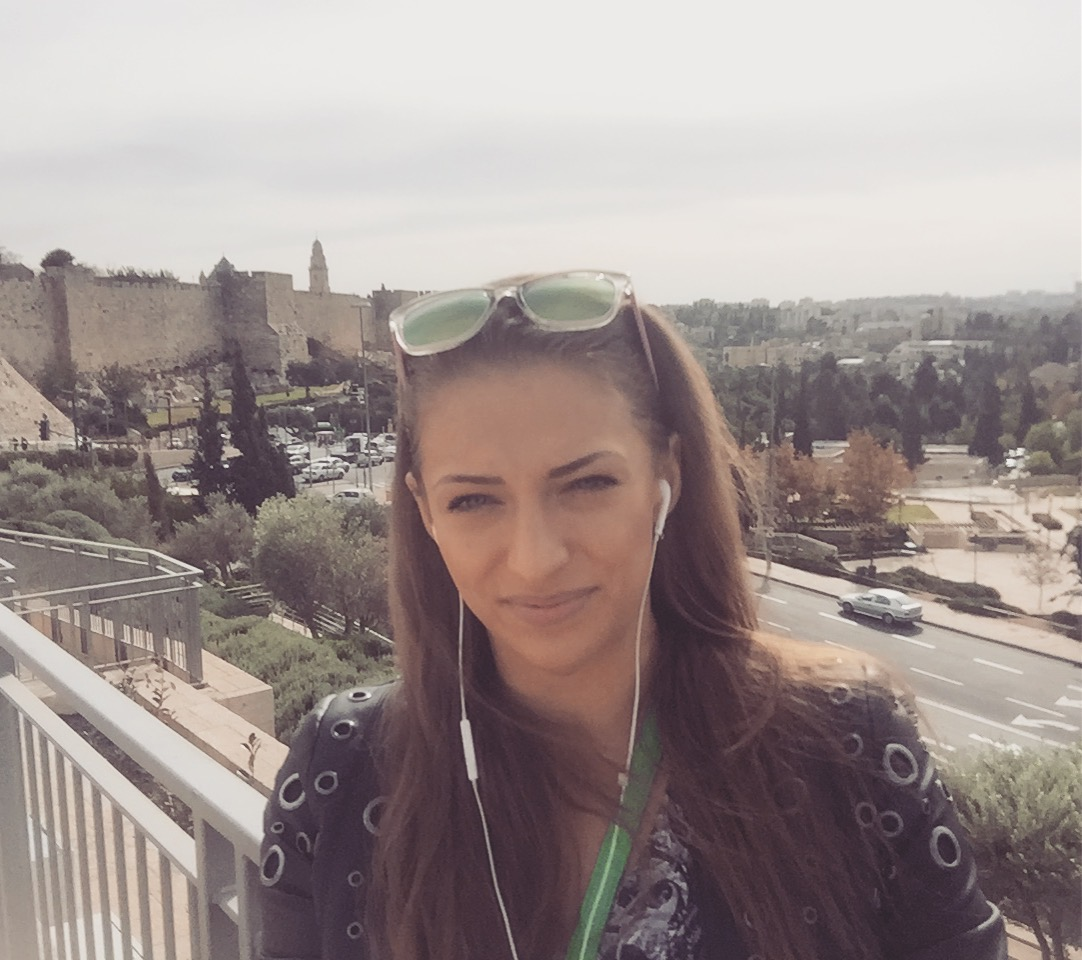
\includegraphics[scale=0.25]{Photo1}
\subsection{Факты обо мне:}
\begin{enumerate}
\item С 4х лет занимаюсь спортом.
\item Оптимист по жизни.
\item Люблю людей с хорошим чувством юмора.
\item Девиз: "упорство и труд всё перетрут".
\item Продаю свое шоу.
\item Я ответственный человек.
\item Любимая книга "Понедельник начинается в субботу"
\item Сериалы не люблю, но "Игры престолов" и "Breaking Bad"- Исключение.
\item Меломан.
\item Обожаю стеб Кирилла Юрьевича.
\end{enumerate}

\subsection{Формулы:}
\begin{align}
 \lim_{\alpha \to 0}
    \frac{sin\alpha}{\alpha}
    =1; \tag{\ae}\label{aster} \\    
    \int {\ell^x}\, dx
    ={\ell^x}+C;\tag{\ae\ae}\label{aster} \\
    \sum_{i=0}^n a_0*b^i
    =a_0*{\frac{1-b^{n+1}}{1-b}};\tag{\ae\ae\ae}\label{aster}.
    \end{align}
    \begin{align}
   |A|= 
   \begin{pmatrix}
        a_{11} & a_{12} & a_{13} \\
        a_{21} & a_{22} & a_{23}\\
        a_{31} & a_{32}  & a_{33}
    \end{pmatrix}
    &=a_{11}*a_{22}*a_{33}+a_{21}*a_{32}*a_{13}+
    a_{31}*a_{12}*a_{23}-a_{31}*a_{22}*a_{13}-\notag\\
   & a_{21}*a_{12}*a_{33}-a_{11}*a_{32}*a_{23};
    \tag{\ae\ae\ae\ae}\label{aster}.
\end{align}
(\ae);(\ae\ae);(\ae\ae\ae);(\ae\ae\ae\ae): Все гениальное - Просто!
\end{document}